\chapter{Event Reconstruction}

Reconstruction is the process and algorithms that attempt to reform information about collision events and their decay products from detector signals. This process is done at several points in the ATLAS analysis procedure. First partial reconstruction of RoI's is done at the Level-2 trigger while a mostly full detector reconstruction is done at the EF. After the data has been permanently stored full reconstruction of all possible signatures in each event as well as whole event variables can be completed if it failed to finish live during the trigger decision.

The other main source of reconstruction is done in a process called reprocessing. After data has been stored updates to sub-detector calibrations and optimisations can take place and so reconstruction of entire data sets takes place to update variables to more accurate measurements. 

The Data format used in this analysis is an internal ATLAS format called a D3PD. This format is a type of ROOT \cite{Antcheva20092499} ntuple, or sequence of ordered lists, which stores ATLAS event data. The data used has past through ATLAS software reconstruction while the Monte-Carlo (MC) background estimate samples have gone through a GEANT 4 \cite{Agostinelli2003250} detector simulation as well as ATLAS reconstruction. This means analysis of these D3PD's with root requires only minor corrections.


Some of the many variables reconstructed are event specific and one of the more important of this is the number of interactions per bunch crossing. As more than one proton collision takes place with each bunch collision a lot of physics background can appear in an event. This makes the search harder but it is also needs to be predicted properly by background estimates. The problem is referred to as pile-up and corrections needed to accommodate it are discussed in section \ref{sec:correc}. Figure \ref{fig:pu} shows the distribution of number of interactions per bunch crossing seen in the 7 TeV and 8 TeV ATLAS data sets.

\begin{figure}[h!]
	\centering
		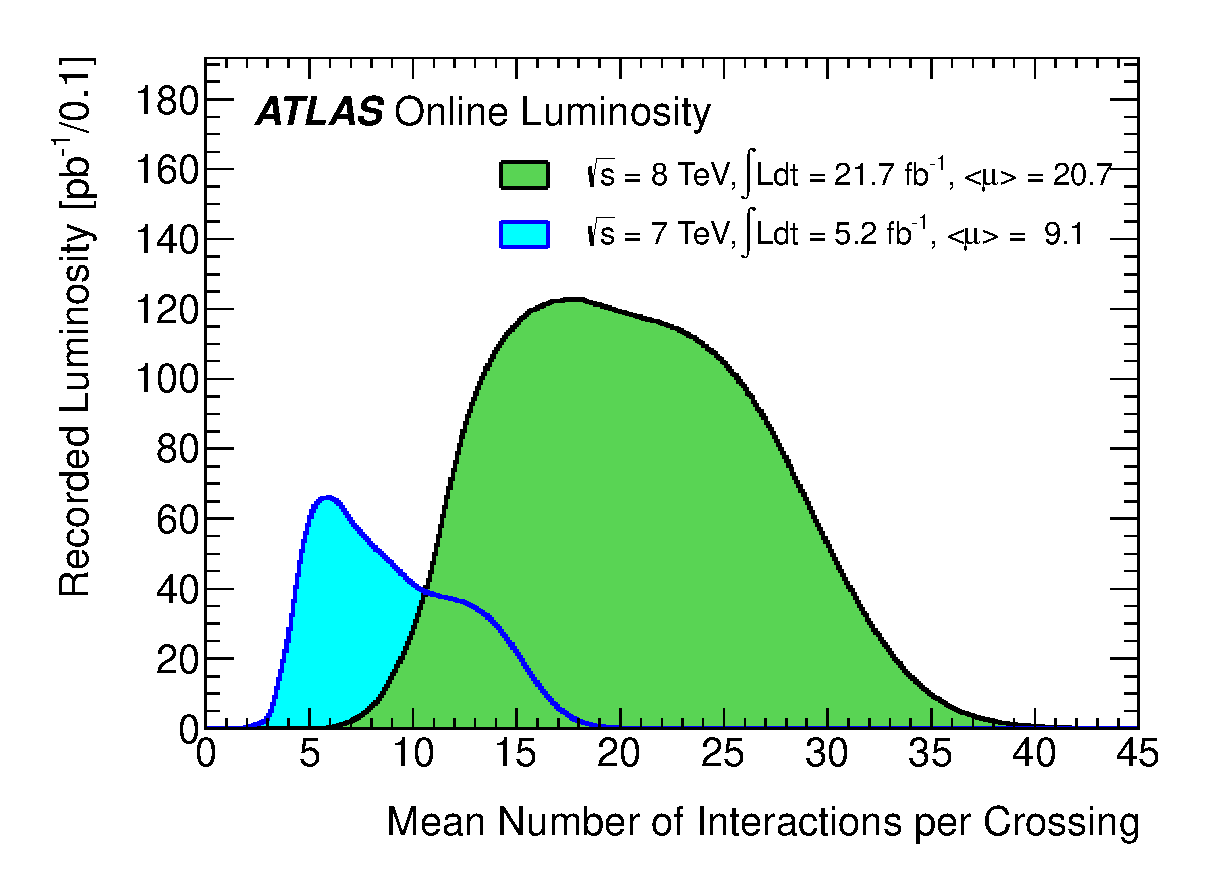
\includegraphics[width=0.8\linewidth]{images/mu_2011_2012-dec.eps}
	\caption{Luminosity-weighted distribution of the mean number of interactions per crossing for the 2011 and 2012 data. \cite{mu_2011_2012_dec,Aad:2011dr}}
	\label{fig:pu}
\end{figure}


Below will mainly be a discussion of the reconstruction of electron (and related photon) objects as these are the decay products searched for in this analysis.



\section{Electron Reconstruction and Identification}
\label{sec:ReconElec}

	During reconstruction each EM calorimeter energy signature with an associated track in the inner detector get listed as an electron object. These objects get selected via a clustering algorithm in the EM calorimeter which defines the energy and is then matched to a track. These objects then have a list of associated variables derived from detector readouts on which an analysis selection for `good' electrons can be made. These variables range from simple values of position and energy to more complex derived values such as isolation. A few variables will be listed below relevant to this analysis and how they are derived.

	\begin{itemize}
	\item $\eta$ \& $\phi$, a particle trajectory or position in detector. These are the main variables for measuring the direction the particle went in the detector and for electrons can be measured in two ways. Either via cluster location in the EM calorimeter or measurement in the inner detector.
	\item $p_{T}$ or transverse momentum. $p_{T}$ is the main measure of energy used for particles where $p_{T}~=~|p|\cosh{\eta}$. Here $\eta$ comes from either the inner detector or calorimeter cluster hit location and the choice is dependent on a how many hits the track made travelling though the inner detector and therefore how accurate the measurement is.
	\item $E_{T}$cone20. This is a cluster isolation variable measuring the sum of energy found around the region of interest minus the electron cluster for $R < 0.20$ where $R = \sqrt{\eta^{2} + \phi^{2}}$. $E_{T}$cone20 is used to check cone isolation in order to eliminate jet like signatures from the analysis which often create large showers in the calorimeters.
	\item Electron Charge. This is simple matter of measuring the direction the electron curves in the inner detector. However as discussed in chapter 5 this can be hard for very high energy electrons.
	\item loose, medium, tight. This is a definition given to a set of selections defining how certain it is the object is an electron. The selections and variables associated with this are discussed below.
	\end{itemize}

	Loose, medium and tight define an increasing series of selections for identifying good electron signatures in the detector. The selections vary between shower shape variables to track quality and track cluster matching. Some of the important associated variables are discussed in table \ref{tab:Rec_lmt} with the full selections found in appendix \ref{ap:em} as the full selections are two dimensional arrays of threshold for most selections. Also to note there are two different definitions of medium referred to as medium and medium++. The latter is a re-optimisation of the selection and slightly stricter than the original medium. medium++ is used in this analysis and found in appendix \ref{ap:em}.

	\begin {table}[h!]
	\begin{center}
  	\begin{tabular}{llc}
		\hline
		\multicolumn{3}{l}{{\bf Loose selection}} 																					\\ 
		%\hline
		Type 				& Description																	& Name 					\\
		\hline
\rule{0pt}{3ex}Acceptance 			& $|\eta|~<~2.47$ 														& $\eta$				\\
\rule{0pt}{4ex}Hadronic leakage	& Ratio of $E_{T}$ in the first layer of the hadronic calorimeter to $E_{T}$ & \multirow{2}{*}{$R_{had1}$}			\\
							& of the EM cluster (used over the range $|\eta|<0.8$ and $|\eta|>1.37$)		&						\\
							\rule{0pt}{3ex} 
							& Ratio of $E_{T}$ in the hadronic calorimeter to $E_{T}$ of the EM cluster 	& \multirow{2}{*}{$R_{had}$}			\\
							& (used over the range $|\eta|~<~0.8$ and $|\eta|~>~1.37$)						&						\\
\rule{0pt}{4ex}Middle layer of  	& Ratio of the energy in $3\times7$ cells over the energy in $7\times7$ cells	& \multirow{2}{*}{$R_{\eta}$}	\\
		EM calorimeter		& centred at the electron cluster position												&						\\
							\rule{0pt}{3ex} 
							& Lateral shower width, $\sqrt{(\sum{E_{i} \eta_{i}^{2}})/(\sum{E_{i}}) - ((\sum{E_{i} \eta_{i}})/(\sum{E_{i}}))^{2}}$,  	& \multirow{3}{*}{$\omega_{\eta2}$}		\\
							& where $E_{i}$ is the energy and $\eta_{i}$ is the pseudorapidity of cell $i$ and & 			\\
							& the sum is calculated  within a window of 3 $\times$ 5 cells								&						\\
		\hline
		\hline
		\multicolumn{3}{l}{{\bf medium \& medium++ selection} (includes loose)}																	\\
		%\hline
		Type 				& Description																	& Name 		 			\\
		\hline
\rule{0pt}{3ex}Strip layer of EM & Shower width, $\sqrt{(\sum{E_{i}(i - i_{max})^{2}})(\sum{E_{i}})}$, where $i$ runs over all & \multirow{4}{*}{$\omega_{stot}$}	\\
		calorimeter 		& strips in a window of $\Delta\eta~\times~\Delta\phi~\approx~0.0625~\times~0.2$, &			\\
							& corresponding typically to 20 strips in $\eta$, and $i_{max}$ is the index 	& 						\\
							& of the highest-energy strip 				&           \\
							\rule{0pt}{3ex}
							& Ratio of the energy difference between the largest and second  		& \multirow{2}{*}{$E_{ratio}$}			\\
							& largest  energy deposits in the cluster over the sum of these 					&						\\
							& energies & \\
\rule{0pt}{4ex}Track quality	& Number of hits in the pixel detector $(\geq1)$							& $n_{pixel}$			\\
							& Number of total hits in the pixel and SCT detectors $(\geq7)$					& $n_{Si}$				\\
							& Transverse impact parameter $(|d_{0}|~<~5~\text{mm})$							& $d_{0}$				\\
\rule{0pt}{4ex}Track-cluster		& $\Delta\eta$ between the cluster position in the strip layer and the  	& \multirow{2}{*}{$\Delta\eta$} 	\\
		matching			& extrapolated track $(|\Delta\eta|~<~0.01)$													& 						\\
		\hline				
		\hline
		\multicolumn{3}{l}{{\bf Tight selection} (includes medium)}																	\\
		%\hline
		Type 				& Description 																	& Name 					\\
		\hline
\rule{0pt}{3ex}Track-cluster		& $\Delta\phi$ between the cluster position in the middle layer and the  & \multirow{2}{*}{$\Delta\phi$}	\\
		matching			& extrapolated track $(|\Delta\phi|~<~0.02)$													& 						\\
							& Ratio of the cluster energy to the track momentum								& $E/p$					\\
							& Tighter $\Delta\eta$ requirement $(|\Delta\eta|~<~0.005)$						& $\Delta\eta$ 			\\
\rule{0pt}{4ex}Track quality		& Tighter transverse impact parameter requirement $(|d_{0}|<1\text{mm})$		& $d_{0}$				\\
		TRT 				& Total number of hits in the TRT 												& $n_{TRT}$				\\
							& Ratio of the number of high-threshold hits to the total number  				& \multirow{2}{*}{$f_{HT}$}				\\
							& of hits in the TRT 																		& 						\\
\rule{0pt}{4ex}Conversions 	& Number of hits in the b-layer $(\leq1)$ 										& $n_{BL}$				\\
							& Veto electron candidates matched to reconstructed  & 						\\
							& photon conversions 		 						 & 						\\
		\hline
  		\end{tabular}
  	\caption{The variables associated with definitions of loose, medium and tight \cite{Aad:2011mk}. Full thresholds found in appendix \ref{ap:em}}
  	\label{tab:Rec_lmt}
  	\end{center}
	\end {table}












